%% img/timespacehierarchies/PaddingCheat.tex
%% Copyright 2019 Andrea Berlingieri
%
% This work may be distributed and/or modified under the
% conditions of the LaTeX Project Public License, either version 1.3
% of this license or (at your option) any later version.
% The latest version of this license is in
%   http://www.latex-project.org/lppl.txt
% and version 1.3 or later is part of all distributions of LaTeX
% version 2005/12/01 or later.
%
% This work has the LPPL maintenance status `maintained'.
%
% The Current Maintainer of this work is Andrea Berlingieri.
%
% This work consists of all files listed in manifest.txt
\documentclass{standalone}

\usepackage{../TikzStyle}
\usepackage{../mystyle}

\newcommand{\gpoint}[2]{%
\filldraw [gray] (#1,#2) circle [radius=2pt]
}

\begin{document}
    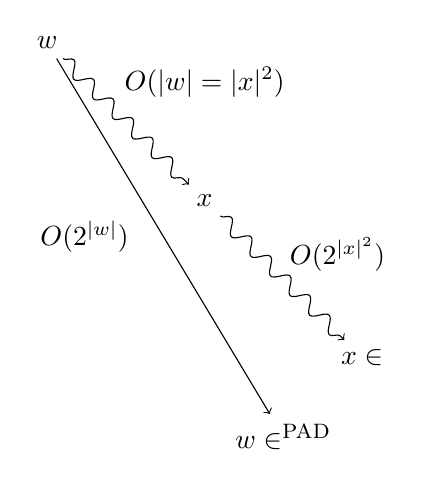
\begin{tikzpicture}
        \node (w) at (0,0) {$w$};
        \node (x) at (2,-2) {$x$};
        \node (xinL) at (4,-4) {$x \in \Lang$};
        \node (winLpad) at (3,-5) {$w \in \Lang^{\textsc{pad}}$};
        \draw[->,decorate,decoration=snake] (w) -- (x) node [pos=0.5,xshift=1cm,yshift=0.5cm]
        {$O(|w| = |x|^{2})$};
        \draw[->,decorate,decoration=snake] (x) -- (xinL) node [pos=0.5,xshift=0.7cm,yshift=0.3cm]
        {$O(2^{|x|^{2}})$};
        \draw[->] (w) -- (winLpad) node [pos=0.5,xshift=-1cm] {$O(2^{|w|})$};
    \end{tikzpicture}
\end{document}
